%%%%%%%%%%%%%%%%%%%%%%%%%%%%%%%%%%%%%%%%%%%%%%%%%%%%%%%%%%%%%%%%%%%%%%%%%%% 
% 
% Generic template for TFC/TFM/TFG/Tesis
% 
% By:
% + Javier Macías-Guarasa. 
% Departamento de Electrónica
% Universidad de Alcalá
% + Roberto Barra-Chicote. 
% Departamento de Ingeniería Electrónica
% Universidad Politécnica de Madrid   
% 
% Based on original sources by Roberto Barra, Manuel Ocaña, Jesús Nuevo,
% Pedro Revenga, Fernando Herránz and Noelia Hernández. Thanks a lot to
% all of them, and to the many anonymous contributors found (thanks to
% google) that provided help in setting all this up.
% 
% See also the additionalContributors.txt file to check the name of
% additional contributors to this work.
% 
% If you think you can add pieces of relevant/useful examples,
% improvements, please contact us at (macias@depeca.uah.es)
% 
% You can freely use this template and please contribute with
% comments or suggestions!!!
% 
%%%%%%%%%%%%%%%%%%%%%%%%%%%%%%%%%%%%%%%%%%%%%%%%%%%%%%%%%%%%%%%%%%%%%%%%%%% 

\chapter{Introduction}
\label{cha:introduction}

\begin{FraseCelebre}
  \begin{Frase}
    Aaay, el oro, la fama, el poder.  \\
    Todo lo tuvo el hombre que en su día se autoproclamó  \\
    el rey de los piratas, ¡GOLD ROGER!  \\
    Mas sus últimas palabras no fueron muy afortunadas:  \\
    "¿¡MI TESORO!? Lo dejé todo allí, buscadlo si queréis,  \\
    ojalá se le atragante al rufián que lo encuentre.
  \end{Frase}
  \begin{Fuente}
    Opening 1 de One Piece: "We are" \\
    Autor original: Hiroshi Kitadani
  \end{Fuente}
\end{FraseCelebre}

\section{Motivation}
\label{sec:1_motivation}

\ac{AD} have held the attention of technology enthusiasts and futurists for some time as is evidenced by the continuous research and development of this topic in \ac{ITS} over the past decades, being one of the emerging technologies of the \textit{Fourth Industrial Revolution}, and particularly of the Industry 4.0. \\

The concept \textit{Fourth Industrial Revolution} or Industry 4.0  was first introduced by Klaus Schwab , CEO (Chief Executive Officer) of the World Economic Forum, in a 2015 article in Foreign Affairs (American magazine of international relations and United States foreign policy). A technological revolution can be defined as a period in which one or more technologies are replaced by other kinds of technologies in a short amount of time. Hence, it is an era of accelerated technological progress featured by Researching, Development and Innovation whose rapid application and diffusion cause an abrupt change in society. In particular, the \textit{Fourth Industrial Revolution} conceptualizes rapid change to industries, technology, processes and societal patterns in the 21st century due to increasing inter-connectivity and smart automation. This industrial revolution focuses on operational efficiency, being the following four themes which summarize it: \\

\begin{itemize}
	\item Decentralized decisions: Ability of cyber physical systems to make decisions on their own and to perform their tasks as autonomously as possible.
	\item Information transparency: Provide operators with comprehensive information to make decisions. Inter-connectivity allows operators to gather large amounts of information and data from all points in the manufacturing process in order to identify key areas or aspects that can benefit from improvement to enhance functionality.
	\item Technical assistance: Ability to assist humans with unsafe or difficult tasks and technological facility of systems to help humans in problem-solving and decision-making.
	\item Interconnection: Ability of machines, sensors, devices and people to communicate and conect with each other via the Internet of Things (IoT) or the Internet of People (IoP).
\end{itemize}

Based on the aforementioned principles, this revolution is expected to be marked by breakthroughs in emerging technologies in fields such as nanotechnology, quantum computing, 3D printing, Internet of Things (IoT), fifth-generation wireless technologies (5G), Robotics, Computer Vision (CV), \ac{AI} or the scope of this PhD thesis, \acp{ADS}. The sum of all these advances are resulting in machines that can potentially see, hear and what is more important, think, moving more deftly than humans. \\

An \ac{ADS}, also referred in the literature as Intelligent Vehicle (IV), driverless car or autonomous car, is a vehicle tan can sense its surrounding and moving safely with little or even no human input. These \acp{ADS} must combine a variety of sensors to understand the traffic scenario, like RADAR (RAdio Detection A Ranging), LiDAR (Light Detection and Ranging), cameras, Inertial Measurement Unit (IMU), wheel odometry, GNSS (Global Navigation Satellite System) or ultrasonic sensors, and detect, track and predict (which is the main purpose of this thesis) the most relevant obstacles around the ego-vehicle. Then, advanced control and planning systems process this sensory information in combination with a predefined global route to calculate the corresponding control commands to drive throughout the environment, ensuring a safe driving. \\

The dream of seeing fleets of \acp{ADS} efficiently delivering goods and people to their destination has fueled billions of dollars and captured consumer's imaginations in investment in recent years. Nevertheless, according to the "Autonomous driving's future: Convenient and connected" report, published by the global management consulting firm McKinsey \& Company in January 2023, even after some setbacks have pushed out timelines for \ac{AD} launches and delayed customer adoption, the transportation community still broadly agrees that \ac{AD} has the potential to transform consumer behaviour, transportation and society at large. \ac{AD} is considered as one of the solutions to the aforementioned problems and one of the greatest challenges of the automotive industry today. \\

Statistics show that 69 \% of the population in the European Union (EU), including associated states, lives in urban areas. According to the World Health Organization, nearly one third of the world population will live in cities by 2030, leading to an overpopulation in most of them. Aware of this problem, the Transport White Paper published by the European Commission in 2011 indicated that new forms of mobility ought to be proposed so as to provide sustainable solutions for people and goods safely. For example, regarding safety, it sets the ambitious goal of halving the overall number of road deaths in the EU between 2010 and 2020. Nevertheless, this goal does not seem to be easy since only in 2014 more than 25,700 people died on the roads in the EU, many of them caused by an improper behaviour of the driver on the road. A similar study made by the National Highway Traffic Safety Administration (NHTSA, tranportation organization of the United States) reported in 2015 that around 94 \% of traffic accidents happen because of human error. In that sense, the existence of reliable and economically affordable \acp{ADS} are expected to create a huge impact on society affecting social, demographic, environmental and economic aspects. It can produce substantial value for the auto industry, drivers and society, making driving safer, more convenient and more enjoyable. While the human driver or not could select whether to drive, in autonomous mode hours on the road previously spent driving could be used to work, watch a funny movie or even to video call a friend. For employees with long commutes, \ac{AD} might shorten the workday, increasing worker productivity. Since workers, specially those related to digital jobs or related fields, may perform their jobs from an \ac{ADS}, they could more easily move further away from the office, which, in turn, could attract more people to suburbs and rural areas. Besides this, it is estimated to cause a reduction in road deaths, reduce fuel consumption and harmful emission associated and improve traffic flow, as well as an improvement in the overall driver comfort and mobility in groups with impaired faculties, such as disable or elderly people, providing them with mobility options that go beyond car-sharing services or public transportation. Other industrial applications of autonomous vehicles are agriculture, retail, manufacturing, commercial and freight transport or mining. \\

\section{Historical Context}
\label{sec:1_historical_context}

\acp{ADS} have become a challenge for auto competitions and technology companies, which has derived in an intense competition. Though today companies such as Mercedes, Ford or Tesla are racing to build \acp{ADS} for a radically changing consumer world, the research and development of autonomous robots is not new. \\

In 1500, centuries before the invention of the automobile, Leonardo da Vinci designed a cart that could move without being pulled or pushed. In 1868, Robert Whitehead invented a torpedo that could propel itself underwater in order to be a game-changer for naval fleets all over the world. In terms of robotic solutions for intelligent mobility, the study was started in the 1920s, being the concept of Autonomous Car defined in Futurama, an exhibit at the 1939 New York Wolrd's Fair. General Motors created the exhibit to display its vision of what the world would look like in 20 years, including an automated highway system that would guide \ac{ADS}. By 1958, General Motors made this concept a reality (at least as a proof of concept) being the car's front end embedded with sensors to detect the current flowing through a wire embedded in the road. The first semi-automated car was developed in 1977 by Japan’s Tsukuba Mechanical Engineering Laboratory. The vehicle reached speeds up to 30 km/h with the support of an elevated rail. \\

\begin{figure}[h]
	\centering
	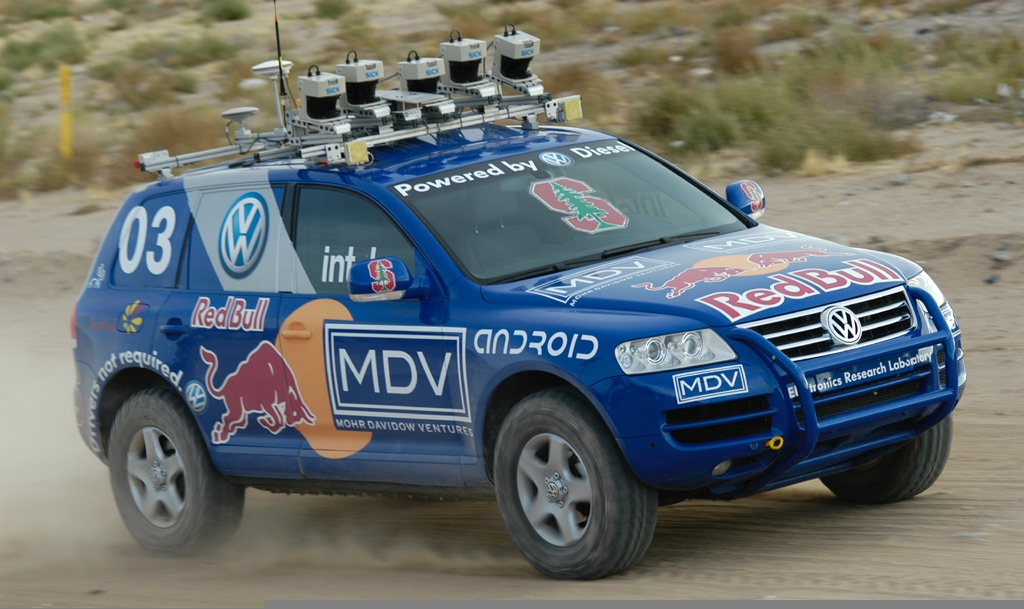
\includegraphics[width=0.8\linewidth]{1_darpa_winner_2005.png}
	\caption{Stanley, 2005 DARPA Grand Challenge winner}
	Source: \textit{Stanford university}
	\label{fig:1_darpa_winner_2005}
\end{figure}

Nevertheless, the first truly autonomous cars appeared in the 1980s with Carnegie Mellon University’s Navlab and ALV projects funded by the USA company DARPA (Defense Advanced Research Projects Agency) in 1984 and EUREKA Prometheus project (1987) developed by Mercedes-Benz and Bundeswehr University Munich’s. By 1985, the ALV project had shown self-driving speeds on two-lane roads of 31 km/h with obstacle avoidance added in 1986 and off-road driving in day and night conditions by 1987. Furthermore, from the 1960s through the second DARPA Grand Challenge in 2005 (212 km off-road course near the California-Nevada state line, surpassed by all but one of the 23 finalists), automated vehicle research in the United States was primarily funded by DARPA, the US Army and US Navy, yielding rapid advances in terms of speed, car control, sensor systems and driving competence in more complex conditions. This caused a boost in the development of autonomous prototypes by companies and research organizations, most of them from the United States. Figure \ref{fig:1_darpa_winner_2005} shows Stanley, the 2005 DARPA Gran Challenge winner, from Stanford university. \\

Even though self-driving cars have not yet displaced conventional cars, there can be found several examples of how it has become a hot topic for powerful companies such as Delphi Automotive Systems, Audi, BMW, Tesla, Mercedes-Benz or Waymo. \\

In 2005 Delphi broke the Navlab’s record achievement (driving 4,584 km while remaining 98 \% of the time autonomously) by piloting an Audi, improved with Delphi technology, over 5,472 km through 15 states while remaining in self-driving mode 99 \% of the time. Moreover, in 2005 the USA states of Michigan, Virginia, California, Florida, Nevada and the capital, Washington D.C., allowed the testing of automated cars on public roads. \\

In 2017, Audi stated that its A8 car prototype would be automated at speeds up to 60 km/h by using its perception system named “Audi AI”.  Also, in 2017 Waymo (self-driving technology development company subsidiary of Alphabet Inc) started a limited trial of a self-driving taxi service in Phoenix, Arizona. \\

Figure \ref{fig:1_disengagement_2020} shows the total number of autonomous test miles and miles per disengagement in California (Dec 2019 - Nov 2020) by some of the most important \ac{AD} technology development companies around the world. The concept disengagement is quite useful to assess the quality of an \ac{ADS}, defined as the deactivation of the autonomous mode when a failure of the autonomous technology is detected or when a safe operation requires that the autonomous vehicle test driver disengages the autonomous mode, resulting in control being seized by the human driver.

\begin{figure}[ht]
	\centering
	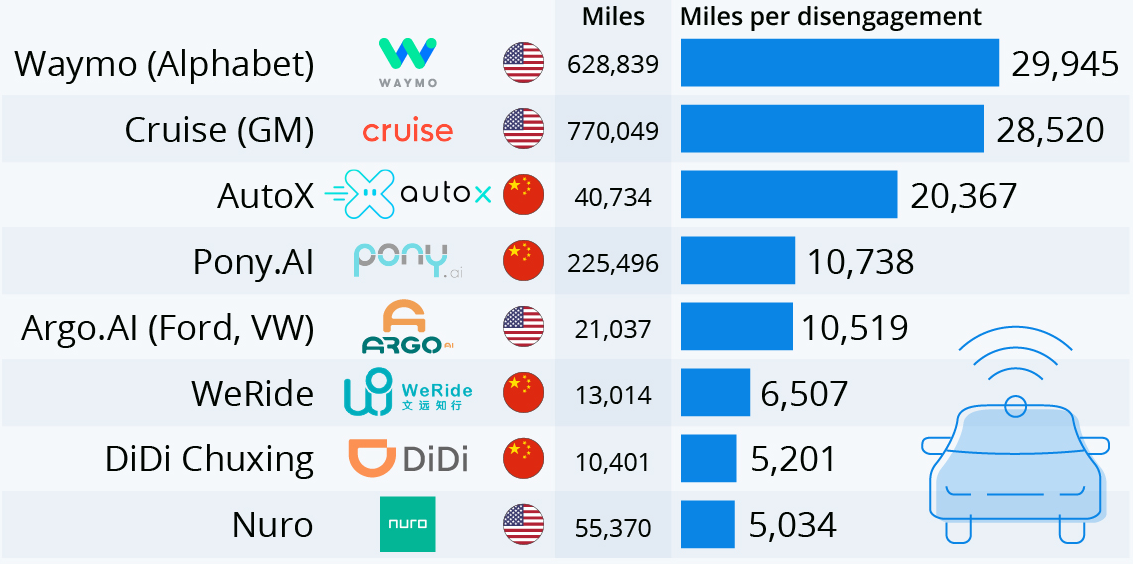
\includegraphics[width=0.6\linewidth]{1_disengagement_2020.png}
	\caption{Number of autonomous test miles and miles per disengagement (Dec 2019 - Nov 2020)}
	Source: \textit{DMV California, via The Last Driver License Holder}
	\label{fig:1_disengagement_2020}
\end{figure}

At the moment of writing this thesis (2023), many vehicles on the road are considered to be semi-autonomous due to safety features like braking systems, assisted parking, lane boundaries detection or predict the long-term behaviour of the users around the vehicle to execute the most optimal action in a safely way. Regarding this, the Society of Automotive Engineers (SAE) published the concept of autonomy levels in 2014, as part of its "Taxonomy and Definitions for Terms Related to On-Road Motor Vehicle Automated Driving Systems" report. Figure \ref{fig:1_nhtsa_sae_automation_levels} illustrates the six levels of autonomy (the higher the level, the more autonomous the car is), where it can be appreciated that Level Zero means "No Automation", being the acceleration, braking and steering controlled by a human driver at all times, and Level Five represents Full Automation, where there is a full-time automation of all driving tasks on any road, under any conditions, whether there is a human on board or not.

\begin{figure}[h]
	\centering
	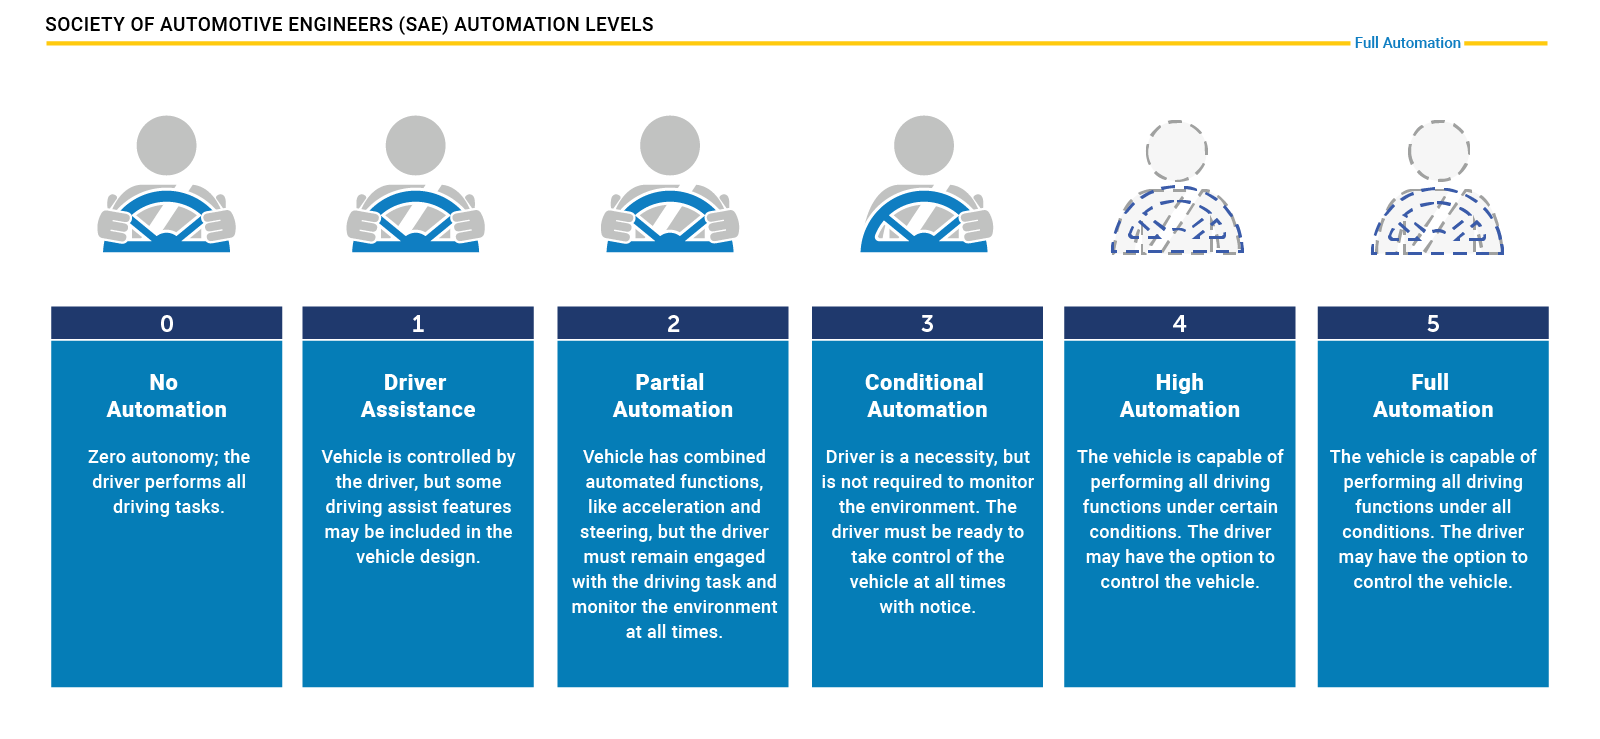
\includegraphics[width=0.8\linewidth]{1_nhtsa_sae_automation_levels.png}
	\caption{Society of Automotive Engineers (SAE) automation levels}
    Source: \textit{NHTSA (National Highway Traffic Safety Administration)}
	\label{fig:1_nhtsa_sae_automation_levels}
\end{figure}

In that sense, today most vehicles only included basic Advanced Driver Assistance Systems (ADAS), but major advancements in AD capabilities are on the horizon. According to a 2021 McKinsey consumer survey, growing demand for \ac{AD} systems could create billions of dollars in revenue. Based on a consumer interest in \ac{AD} features and commercial solutions available on the market today, ADAS and AD could generate between \$300 and \$400 billions in the passenger car market by 2035. Figure \ref{fig:1_mckinsey_revenues_ad} illustrates an interesting study reporting the revenues of ADAS and AD from Level 1 (Driver Assistance) to Level 4 (High Automation). As expected, Level 5 is excluded from this study due to the huge difficulties the automotive companies would have to face to adapt their systems under totally different environmental conditions.

\begin{figure}[h]
	\centering
	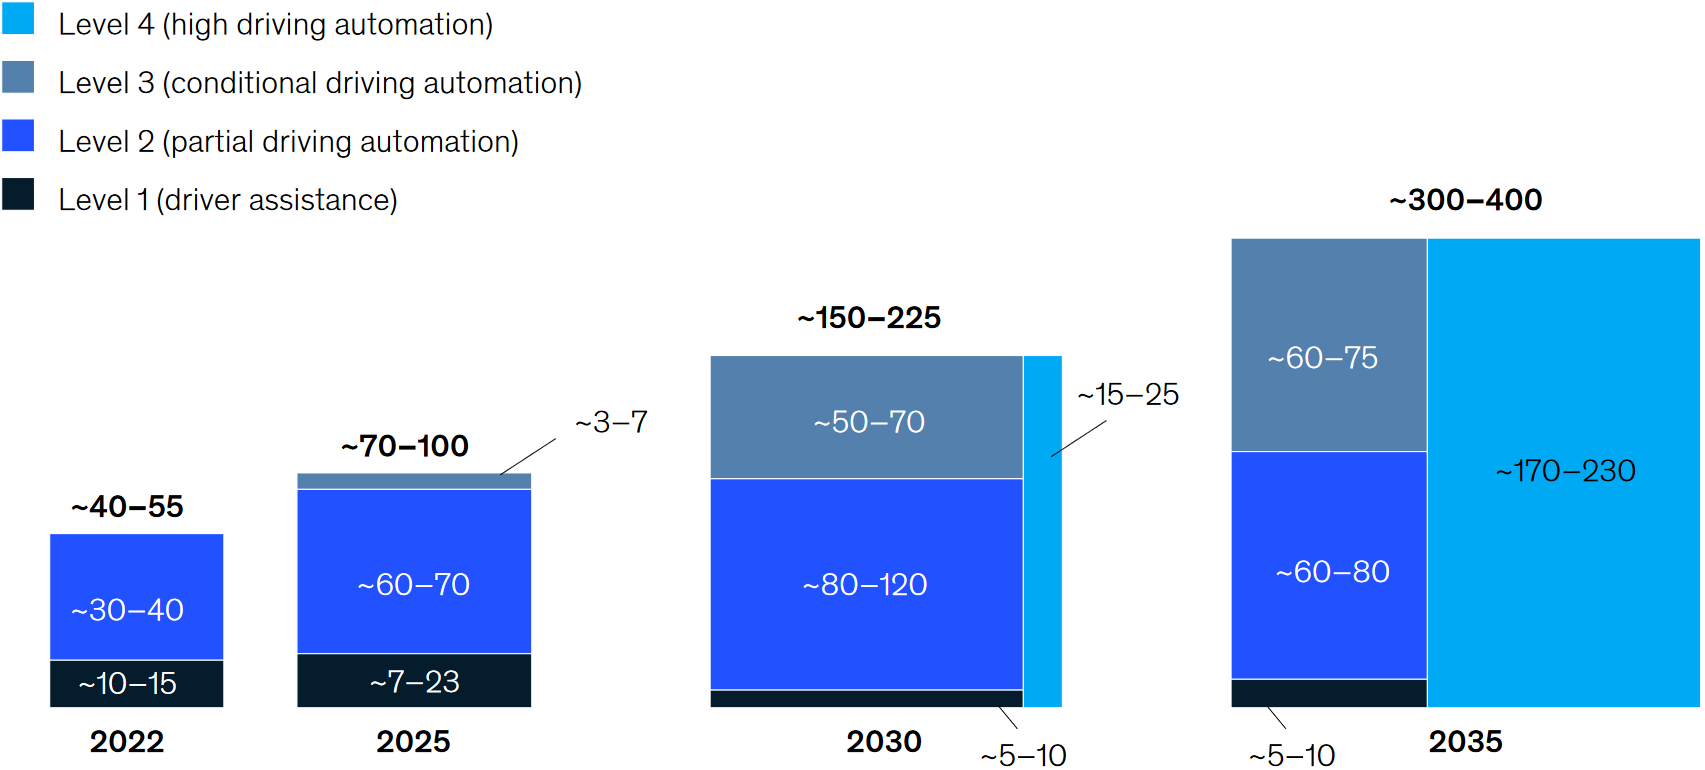
\includegraphics[width=0.8\linewidth]{1_mckinsey_revenues_ad.png}
	\caption{Advanced Driver Assistance systems (ADAS) and \\ Autonomous Driving (AD) revenues in \$ billion} Source: \textit{McKinsey Center for Future Mobility}
	\label{fig:1_mckinsey_revenues_ad}
\end{figure}

\section{Autonomous Driving architecture}
\label{sec:1_ad_architecture}

To sum up what commented above, increasing the level of autonomous navigation in mobile robots (from agriculture to public and private transport) are expected to create tangible business benefits to those users and companies employing them. However, designing an autonomous navigation system does not seem to be an easy task. In the \ac{SOTA} we can distinguish two main kind of software architectures: End-to-End and modular. Figure \ref{fig:1_ete_modular} illustrates the entire \ac{AD} architecture starting from sensing, all the way to longitudinal (throttle/brake) and lateral (steering angle) control of the vehicle, which are the commanded signals that feed the low-level electronic system that moves the vehicle, like a drive-by-wire system \cite{arango2020drive}. End-to-End are considered black-box models, where a single neural network performs the driving task (throttle/steering/brake) from raw sensor data, in such a way the error be may vanished since intermediate representations are jointly optimized, but these are not very interpretable. On the other hand, modular architectures (considered as glass models as counterpart to End-to-End approaches) separate the driving task into individually programmed or trained modules. This solution is more interpretable, since the know-how of a research group or company is easily transferred, they allow parallel development, being the standard solution in industrial research, but the error is propagated, where intermediate representations can led to suboptimal performance. For example, incorrect object detection can lead to low-quality tracking and motion prediction.

\begin{figure}[h]
	\centering
	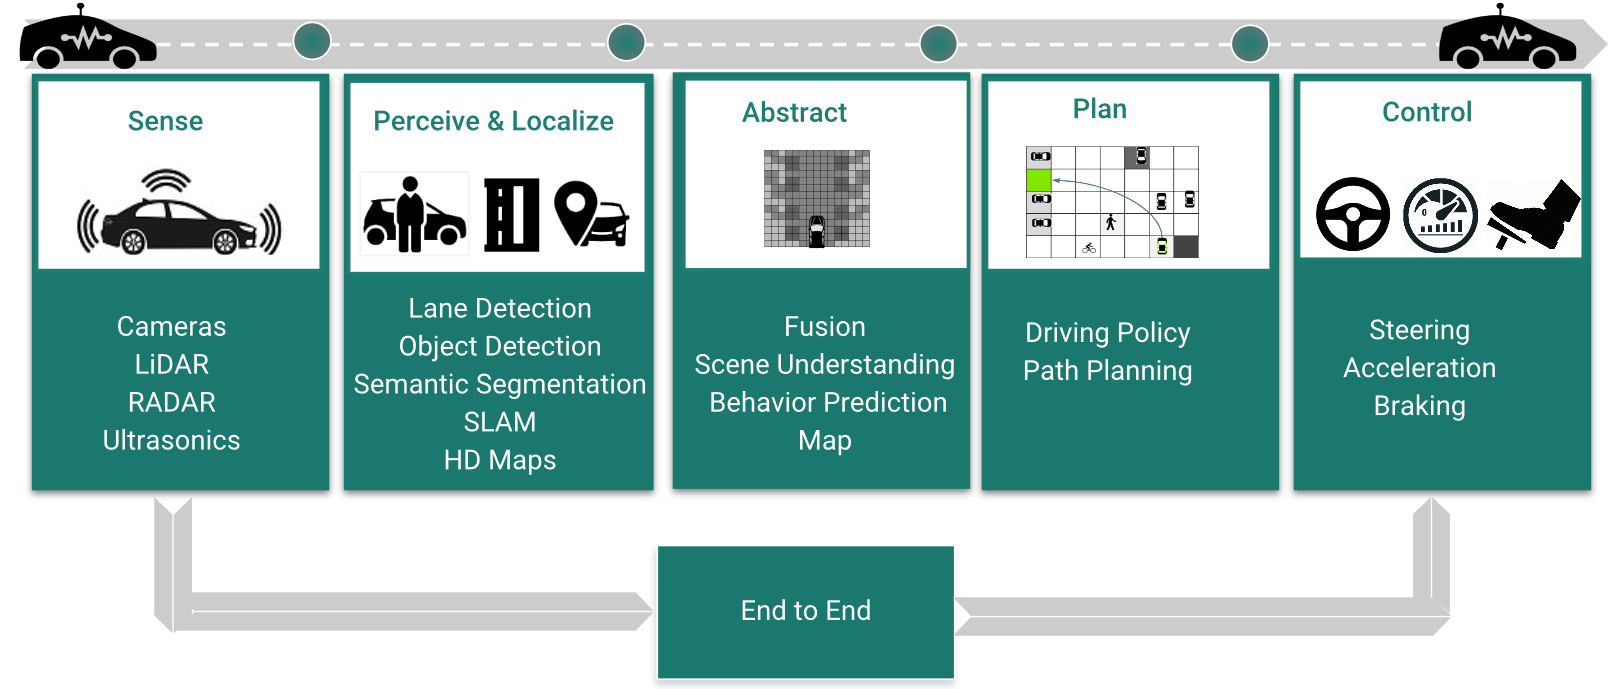
\includegraphics[width=0.8\linewidth]{1_ete_modular.png}
	\caption{Autonomous Driving Stack (ADS) modular vs end-to-end pipeline}
	Source: \textit{Vrunet: Multi-task learning model for intent prediction of vulnerable road users} \cite{ranga2020vrunet}
	\label{fig:1_ete_modular}
\end{figure}

Considering the RobeSafe (Robotics and eSafety) research group and the main projects (Techs4AgeCar, AIVATAR) where this thesis has been developed, we integrate our algorithms in a software modular approach. An example of a software modular approach is shown in Figure \ref{fig:1_pylot_architecture}. Despite the fact in literature some authors disagree on the specific software architecture of an \ac{ADS}, specially the motion prediction module, which is usually classified as a perception algorithm but sometimes is included as part of the planning or decision-making layers, we can hierarchically break down (from raw data to the driving task) a standard \ac{AD} architecture into the following software layers:

\begin{itemize}
	\item Localization layer: Positions and locates the vehicle on a map with real-time and centimetric accuracy approach. The main source of information is a robust differential-GNSS, though IMUs, wheel odometry and even cameras are commonly employed. 
	\item Perception layer: Understand the environment around the ego-vehicle thanks to the information collected by the sensors. If defined as multi-stage, the perception layer first detects the most relevant obstacles, then track them over time to finalize long-term predict with plausible predictions. In order to perform object detection, LiDAR, camera and RADAR are the main sensors that provide the corresponding raw data. Additionally, HD map information is frequently used in the motion prediction tasks by most \ac{SOTA} algorithms.
	\item Mapping layer: Responsible for creating a topologic, semantic and geographical modeling of the environment through which the vehicle drives, being the HD Map graph the most common source of information.
	\item Planning layer: This layer is comprised of three components: route, behaviour and trajectory planner. The route planner computes the most optimal (in terms of distance, time and so forth and so on) global route from some predefined start and goal. It uses the localization and mapping output. On the other hand, the behaviour planner, also referred as decision-making layer by some authors, it performs high-level decision-making of driving behaviours such as lane changes or progress through intersections, mostly focused on the previously computed global route and current localization. It can be seen as an atomization of the global route in different behaviors to reach the goal. Finally, the trajectory planner, also known as local planner, generates a time schedule for how to follow a path given constraints such as position, velocity and acceleration in order to meet the previously decided behaviour and taking into account the prediction from the perception layer, avoiding obstacles in optimal direction and speed conditions.
	\item Control layer: Once the local plan is calculated, the control layer is responsible for generating the commands that are sent to the actuators. It receives as input some waypoints from the calculations made in the trajectory planner. Once these waypoints are received, most authors perform spline interpolations and a velocity profile that ensures a smooth and continous trajectory. 
\end{itemize}

\begin{figure}[h]
	\centering
	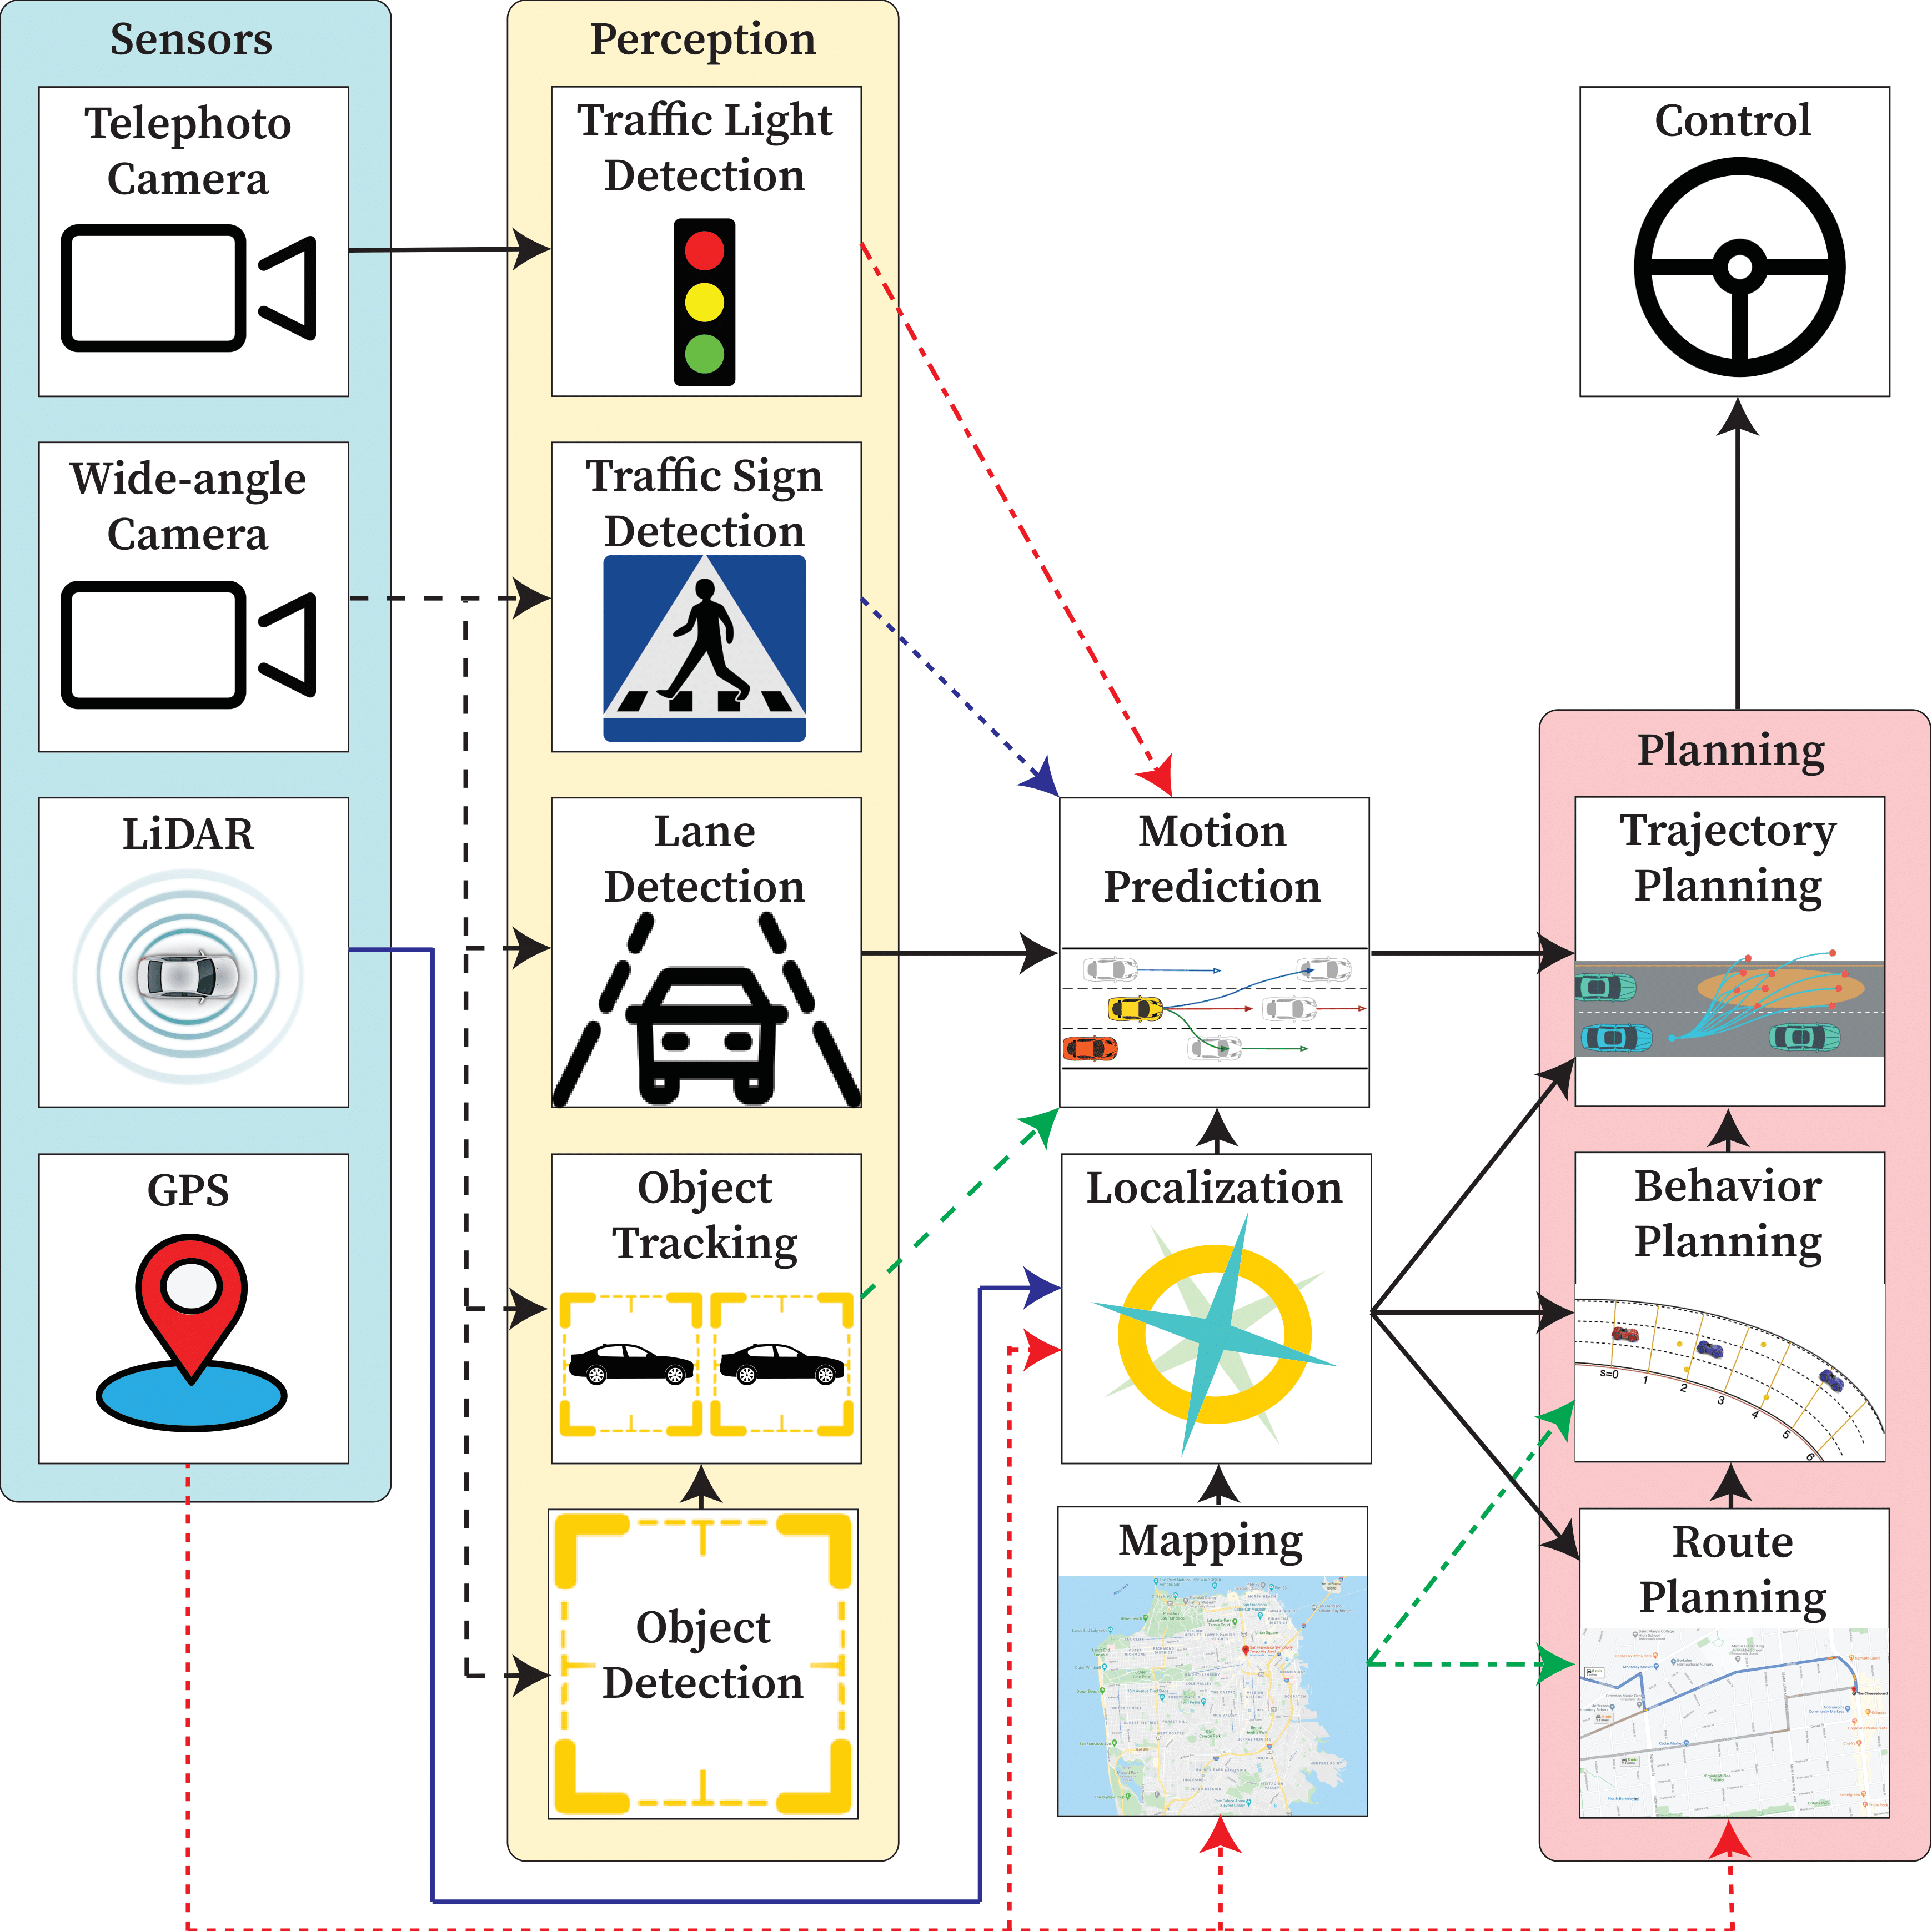
\includegraphics[width=0.8\linewidth]{1_pylot_architecture.png}
	\caption{Autonomous Driving Stack (ADS) modular pipeline}
	Source: \textit{Pylot: A modular platform for exploring latency-accuracy tradeoffs in autonomous vehicles} \cite{gog2021pylot}
	\label{fig:1_pylot_architecture}
\end{figure}

\section{Problem statement}
\label{sec:1_problem_statement}

As commented in previous sections, in order to operate efficiently and safely in highly dynamic, complex and interactive driving scenarios, \acs{ADS} need to smartly reason like human beings via predicting future motions of surrounding traffic participants during navigation. Nevertheless, achieving accurate and robust \ac{MP} in one of the most difficult and interesting challenges to achieve full-autonomy, since it is equivalent to a bridge between the former stages of the perception layer, where the scene is understood detecting and tracking static and dynamic objects of the environment, and the planning and control layer, where the future trajectory of the ego-vehicle is computed and the driving commands are sent to the physical layer (e.g. Drive-by-Wire \cite{arango2020drive}). Here are some of the most important challenges: 

\begin{enumerate}
	\item Heterogeneity of traffic participants. Traffic partipants (specially those which are dynamic) can be roughly classified as cyclists, pedestrians or other vehicles. The prediction model should be capable of differentiating the motion patterns of heterogeneous traffic participants, in such a way fine-grained classification (detection module) is quite beneficial to include additional metadata along with the past observations.
	\item Complexity of road structure. Road structures are highly diverse and complex, specially in highways and urban areas, which noticeably affect the motion behaviours of traffic participants.
	\item Variable number of interactive agents. The prediction model must deal with a number of associated traffic participants within a certain area that can vary from time to time, such as intersections or roundabouts. Then, while driving, a comprehensive representation of the scene must be able to accommodate an arbitrary number of involved traffic participants.
	\item Multimodality of driving behaviours. In real-world, despite we know the behaviour our vehicle will carry out, the motion patterns of other traffic participants can be considered inherently multimodal since there is usually more than one reasonable option for a driver to choose, specially in intersections, when the number of lanes increases or even in the same lane with different velocity profiles (constant velocity, sudden break, sudden acceleration). In that sense, a robust and reliable \ac{MP} model is expected to be human-like and capture different plausible motion modalities where an agent can travel in the prediction horizon.
	\item Complex interpendencies among traffic participants and road infrastructure. Agent-Agent, Agent-Road and Road-Road interpendencies are of great importance for \ac{MP} and interaction modeling, even more taking into account the complexity of road structures and heterogeneity of traffic participants aforementioned. As expected, an agent future trajectory will be affected not only by its own past trajectory and driving objectives (given by the behaviour planner) but also by other surrounding agents past trajectories, traffic rules and physical constraints.
\end{enumerate}

\section{Objectives and Structure of this Thesis}
\label{sec:1_objectives_and_structure}

The main scope of this thesis is to study the \ac{SOTA} and development of novel and efficient interaction-aware Deep Learning based \ac{MP} models, focusing on long-term (from 3 to 6 s) prediction horizon and \ac{AD}, where traffic participants can range from trucks to pedestrians, instead of models focused on pedestrian trajectory prediction. The main inputs that will be used throughout this work are the physical (map) information and historical states (that may include agent position, velocity, orientation, object type and category) of traffic participants in \ac{BEV}, assuming these objects have been previously tracked by our ego-vehicle (also referred as the autonomous car). Though the evaluation of these methods will be done using a single target agent, as proposed by some of the most important prediction datasets, like Argoverse 1 \cite{chang2019argoverse} and Argoverse 2 \cite{wilson2023argoverse}, some of the proposed methods will be trained considering multi-agent. In this thesis, the solutions to the aforementioned challenges will be discussed and investigated progressively. In order to achieve the main scope, the following objectives will be met:

\begin{enumerate}
	\item Research of \ac{SOTA} \ac{MP}, focused on \ac{DL} and the \ac{AD} paradigm.
	\item Propose of several \ac{MP} architectures, studying the progressive incorporation of \ac{DL} mechanisms and different sources of information and metadata, achieving \ac{SOTA} accuracy while reducing in millions of parameters previous models as well as inference time.
	\item Validate the proposed models in downstream applications, such as decision-making or behaviour planning, taking into account former stages of the perception layer (detection and tracking) instead of static files (benchmarks) in hyper-realistic simulation, as a preliminary stage before implementing it in a real-world vehicle.
\end{enumerate}

The organization of this document has been done as follows:

\begin{itemize}
	\item Chapter 2 reviews the most important features and methods of physics-based and learning-based \ac{MP} methods. The physics-based methods are reviewed according to a taxonomy similar to existing reviews. The learning-based methods are reviewed based on two classification criteria: scene representation and trajectory decoding.
	\item Chapter 3 presents a technical background, mostly focused on \ac{DL} mechanisms to deal with temporal sequences and interactions, to deeply understand the proposed methods.
	\item Chapter 4 illustrates the different prediction models developed in the thesis using different validation environments, from unimodal physic-based prediction to the final model of the thesis which takes into account agents interactions, map information and past observations using a novel scene representation with heuristic proposals, graph-based encoding, \ac{DL}-based goal proposals and motion refinement.
	\item Chapter 5 addresses the integration of the final model of the thesis with upstream and downstream modules to contribute the entire pipeline and closed-loop for \ac{AD}.
	\item Chapter 6 summarizes the thesis and provides some promising directions for future work in the areas of \ac{MP} and validation.
\end{itemize}
